%!TEX root = ../larxxia.tex


\section{Introduction to eigenvalues and eigenvectors}
\label{sec:iee}
\secttoc
\index{eigenvalue|(}
\index{eigenvector|(}

\begin{comment}
\pooliv{\S4.1} \layiv{\S5.1} \holti{\S6.1}  \cite[Ch.~8, 11]{Chartier2015}
\end{comment}


This chapter focuses on some marvellous properties of symmetric matrices.  
Nonetheless it defines some basic concepts which also apply to general matrices.  
\cref{ch:gee} explores analogous properties for such general matrices.
The marvellously useful properties developed here result from asking for which vectors does multiplication by a given matrix simply stretch or shrink the vector, without \text{changing direction.}


\begin{definition} \label{def:evecval}
Let \(A\) be a \idx{square matrix}.  
A \idx{scalar}~\(\lambda\) (lambda) is called an \bfidx{eigenvalue} of~\(A\) if 
there is a nonzero vector~\xv\ such that \(A\xv=\lambda\xv\)\,. 
\footnote{The prefix ``eigen-'' comes from the German word for `owning' or `belonging to' in relation to the originating matrix. }
Such a vector~\xv\ is called an \bfidx{eigenvector} of~\(A\) corresponding to the eigenvalue~\(\lambda\).   
\end{definition}


\begin{example} \label{eg:eig3intro}
Consider the \idx{symmetric matrix}
\begin{equation*}
A=\begin{bmatrix} 1&-1&0\\-1&2&-1\\0&-1&1 \end{bmatrix}.
\end{equation*}
\begin{enumerate}
\item Verify an eigenvector is \((1,0,-1)\).  
What is the corresponding eigenvalue?
\begin{solution} 
The simplest approach is to multiply the matrix by the given vector and see what happens.
For vector \(\xv=(1,0,-1)\),
\begin{equation*}
A\xv=\begin{bmatrix} 1&-1&0\\-1&2&-1\\0&-1&1 \end{bmatrix}
\begin{bmatrix} 1\\0\\-1 \end{bmatrix}
=\begin{bmatrix} 1\\0\\-1  \end{bmatrix}
=1\cdot\xv\,.
\end{equation*}
Hence \((1,0,-1)\) is an eigenvector of~\(A\) corresponding to the eigenvalue \(\lambda=1\)\,. 
\end{solution}

\item Verify that \((2,-4,2)\) is an eigenvector.  
What is its corresponding eigenvalue.
\begin{solution} 
For vector \(\xv=(2,-4,2)\),
\begin{equation*}
A\xv=\begin{bmatrix} 1&-1&0\\-1&2&-1\\0&-1&1 \end{bmatrix}
\begin{bmatrix} 2\\-4\\2 \end{bmatrix}
=\begin{bmatrix} 6\\-12\\6  \end{bmatrix}
=3\cdot\xv\,.
\end{equation*}
Hence \((2,-4,2)\) is an eigenvector of~\(A\) corresponding to the eigenvalue \(\lambda=3\)\,. 
\end{solution}

\item Verify that \((1,2,1)\) is not an eigenvector.
\begin{solution} 
For vector \(\xv=(1,2,1)\),
\begin{equation*}
A\xv=\begin{bmatrix} 1&-1&0\\-1&2&-1\\0&-1&1 \end{bmatrix}
\begin{bmatrix} 1\\2\\1 \end{bmatrix}
=\begin{bmatrix} -1\\2\\-1  \end{bmatrix}
\not\propto\begin{bmatrix} 1\\2\\1 \end{bmatrix}.
\end{equation*}
If there was a constant of proportionality (an eigenvalue), then the first component would require the constant \(\lambda=-1\) but the second component would require \(\lambda=+1\) which is a contradiction.
Hence \((1,2,1)\) is not an eigenvector of~\(A\). 
\end{solution}

\item Use inspection to guess and verify another eigenvector (not proportional to either of the above two).  
What is its eigenvalue?
\begin{solution} 
Inspection is useful if it is quick: here one might quickly spot that the \idx{elements} in each row of~\(A\) sum to the same thing, namely zero, so  try vector \(\xv=(1,1,1)\)\,:
\begin{equation*}
A\xv=\begin{bmatrix} 1&-1&0\\-1&2&-1\\0&-1&1 \end{bmatrix}
\begin{bmatrix} 1\\1\\1 \end{bmatrix}
=\begin{bmatrix} 0\\0\\0  \end{bmatrix}
=0\cdot\xv\,.
\end{equation*}
Hence \((1,1,1)\) is an eigenvector of~\(A\) corresponding to the eigenvalue \(\lambda=0\)\,. 
\end{solution}

\end{enumerate}
\end{example}



\begin{activity}
Which of the following vectors is an eigenvector of the \idx{symmetric matrix} \(\begin{bmatrix} -1&12\\12&6 \end{bmatrix}\)?
\actposs[4]{\(\begin{bmatrix} 4\\-3 \end{bmatrix}\)}
{\(\begin{bmatrix} -3\\1 \end{bmatrix}\)}
{\(\begin{bmatrix} -1\\2 \end{bmatrix}\)}
{\(\begin{bmatrix} 2\\1 \end{bmatrix}\)}
\end{activity}



Importantly, eigenvectors tell us key directions of a given matrix: the directions in which the multiplication by a matrix is to simply stretch, shrink, or reverse by a factor: the factor being the corresponding eigenvalue.
In two dimensional plots we can graphically estimate eigenvectors and eigenvalues.
For some examples and exercises we plot a given vector~\xv\ and join onto its head the vector~\(A\xv\): 
\begin{itemize}
\item if both~\xv\ and~\(A\xv\) are aligned in the same direction, or opposite direction, then \xv~is an eigenvector; 
\item if they form some other angle, then \xv~is not an eigenvector.
\end{itemize}
  

\begin{example}   \label{eg:eig2sym}
Let the matrix \(A=\begin{bmat} 1&-1/2\\-1/2&1 \end{bmat}\). 
The plot below-left shows the vector \(\xv=(1,\tfrac12)\), and adjoined to its head the \idx{matrix-vector product} \(A\xv=(\frac34,0)\): 
because the two are at an angle, \((1,\frac12)\)~is not \text{an eigenvector.}
\begin{center}
\begin{tabular}{cc}
\begin{tikzpicture} 
\begin{axis}[footnotesize%,font=\footnotesize
    ,axis equal image, axis lines=middle, thick
    ,ymax=1.5,xtick={0.5,1,1.5},ytick={0.5,1,1.5}]
    \addplot[quiver={u=1,v=0.5},blue,-stealth] 
    coordinates {(0,0)};
    \node[right] at (axis cs:0.4,0.2) {$\xv=(1,\tfrac12)$};
    \addplot[quiver={u=x-0.5*y,v=-0.5*x+y},red,-stealth] 
    coordinates {(1,0.5)};
    \node[above] at (axis cs:1.2,0.5) {$A\xv=(\frac34,0)$};
\end{axis}
\end{tikzpicture}
&
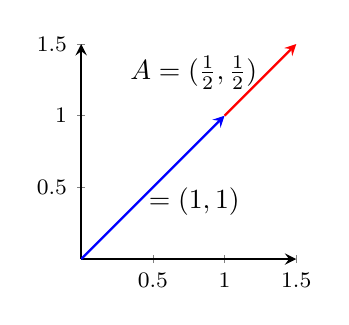
\begin{tikzpicture} 
\begin{axis}[footnotesize%,font=\footnotesize
    ,axis equal image, axis lines=middle, thick
    ,xtick={0.5,1,1.5},ytick={0.5,1,1.5}]
    \addplot[quiver={u=1,v=1},blue,-stealth] 
    coordinates {(0,0)};
    \node[right] at (axis cs:0.4,0.4) {$\xv=(1,1)$};
    \addplot[quiver={u=x-0.5*y,v=-0.5*x+y},red,-stealth] 
    coordinates {(1,1)};
    \node[left] at (axis cs:1.3,1.3) {$A\xv=(\frac12,\frac12)$};
\end{axis}
\end{tikzpicture}
\end{tabular}
\end{center}
However, as plotted above-right, for the vector \(\xv=(1,1)\) the matrix-vector product \(A\xv=(\frac12,\frac12)\) and the plot of these vectors head-to-tail illustrates that they are aligned in the same direction. 
Because of the alignment, \((1,1)\) is an eigenvector of this matrix.
The constant of proportionality is the corresponding eigenvalue: here \(A\xv=(\frac12,\frac12)=\frac12(1,1)=\frac12\xv\) so the eigenvalue is \(\lambda=\frac12\)\,.
This eigenvalue of~\(\frac12\) is seen graphically by the (red) vector~\(A\xv\) being half the length of the (blue) vector~\xv.
\end{example}




\begin{activity} \label{act:eig}
For some matrix~\(A\), the following pictures plot a vector~\xv\ and the corresponding product~\(A\xv\), head-to-tail.
Which picture indicates that~\xv\ is an eigenvector of the matrix?
\actposs[4]{\begin{tikzpicture} 
\begin{axis}[footnotesize%,font=\footnotesize
    ,xmin=-0.5,ymin=-0.5,xmax=2,ymax=2
    ,axis equal image, axis lines=middle ,xtick={0},ytick={0}]
    \twovec{\noexpand\xv}{0.85}{0.52}00
    \twovec{\quad A\noexpand\xv}{0.165}{0.095}{0.85}{0.52}
\end{axis}
\end{tikzpicture}}
{\begin{tikzpicture} 
\begin{axis}[footnotesize%,font=\footnotesize
    ,xmin=-0.5,ymin=-0.5,xmax=2,ymax=2
    ,axis equal image, axis lines=middle ,xtick={0},ytick={0}]
    \twovec{\noexpand\xv}1000
    \twovec{\quad A\noexpand\xv}{0.5}{-0.5}10
\end{axis}
\end{tikzpicture}}
{\begin{tikzpicture} 
\begin{axis}[footnotesize%,font=\footnotesize
    ,xmin=-0.5,ymin=-0.5,xmax=2,ymax=2
    ,axis equal image, axis lines=middle ,xtick={0},ytick={0}]
    \twovec{\noexpand\xv}{0.52}{0.85}00
    \twovec{\quad A\noexpand\xv}{-0.165}{0.59}{0.52}{0.85}
\end{axis}
\end{tikzpicture}}
{\begin{tikzpicture} 
\begin{axis}[footnotesize%,font=\footnotesize
    ,xmin=-0.5,ymin=-0.5,xmax=2,ymax=2
    ,axis equal image, axis lines=middle ,xtick={0},ytick={0}]
    \twovec{\noexpand\xv}0100
    \twovec{\quad A\noexpand\xv}{-0.5}{1}01
\end{axis}
\end{tikzpicture}}
\end{activity}


\begin{activity}
Further, for the picture in \cref{act:eig} that indicates~\xv\ is an eigenvector, is the corresponding eigenvalue~\(\lambda\):
\actposs[4]{\(0.5>\lambda>0\)}{\(\lambda>1\)}{\(1>\lambda>0.5\)}{\(0>\lambda\)}
\end{activity}


As in the next example, we sometimes plot for many directions~\xv\ a diagram of vector~\(A\xv\) adjoined head-to-tail to vector~\xv.
Then inspection estimates the eigenvectors and corresponding eigenvalues \cite[]{Schonefeld1995}.

\needlines9
\begin{wrapfigure}r{0pt}
\def\eRosesize{small}%
\eRose1{-0.5}{-0.5}1
\end{wrapfigure}
\begin{example}[graphical eigenvectors one] \label{eg:eig2pic1}
The plot on the right shows many unit vectors~\xv\  (blue), and for some symmetric matrix~\(A\) the corresponding vectors~\(A\xv\) (red) adjoined. 
Estimate which directions~\xv\ are eigenvectors, and for each eigenvector estimate the corresponding eigenvalue.

(The \script[1]\ function \index{eigshow()@\texttt{eigshow()}}\texttt{eigshow(A)} provides an interactive alternative to this static view.
Download from the internet if using a recent version of \script[1].)

\begin{solution} 
We seek vectors~\xv\ such that~\(A\xv\) is in the same direction (to graphical accuracy).
It appears that vectors at~\(45^\circ\) to the axes are the only ones for which \(A\xv\) is in the same direction as~\xv:  \begin{itemize}
\item the two (blue) vectors \(\pm(0.7,0.7)\) appear to be shrunk to length a half (red) so we estimate two eigenvectors are \(\xv\approx\pm(0.7,0.7)\) and the corresponding eigenvalue  \(\lambda\approx0.5\)\,;
\item the two (blue) vectors \(\pm(0.7,-0.7)\)  appear to be stretched by a factor about~\(1.5\) (red) so we estimate two eigenvectors are \(\xv\approx\pm(0.7,-0.7)\) and the corresponding eigenvalue is \(\lambda\approx1.5\)\,;
\item and for no other (unit) vector~\xv\ is~\(A\xv\) aligned with~\xv.
\end{itemize}
Any multiple of these eigenvectors are also eigenvectors so we may report the directions more simply, perhaps \((1,1)\) and~\((1,-1)\) respectively.
\end{solution}
\end{example}

\needlines6
\begin{wrapfigure}[6]r{0pt}
\def\eRosesize{small}%
\eRose{1}{-0.5}{-0.5}{-0.2}
\end{wrapfigure}
\begin{example}[graphical eigenvectors two] \label{eg:eig2pic2}
The plot on the right shows many unit vectors~\xv\  (blue), and for some symmetric matrix~\(A\) the corresponding vectors~\(A\xv\) (red) adjoined. 
Estimate which directions~\xv\ are eigenvectors, and for each eigenvector estimate the corresponding eigenvalue.

\begin{solution} 
We seek vectors~\xv\ such that~\(A\xv\) is in the same direction (to graphical accuracy):  \begin{itemize}
\item the two (blue) vectors \(\pm(0.9,-0.3)\) appear stretched a little by a factor about~\(1.2\) (red) so we estimate eigenvectors are \(\xv\propto(0.9,-0.3)\) and the corresponding eigenvalue is \(\lambda\approx1.2\)\,;
\item the two (blue) vectors \(\pm(0.3,0.9)\)  appear shrunk and \emph{reversed} by a factor about~\(0.4\) (red) so we estimate  eigenvectors are \(\xv\propto(0.3,0.9)\) and the corresponding eigenvalue is \(\lambda\approx-0.4\)\,---negative because the direction is reversed;
\item and for no other (unit) vector~\xv\ is~\(A\xv\) aligned with~\xv.
\end{itemize}
If this matrix arose in the description of forces inside a solid, then the forces would be compressive in directions~\(\pm(0.3,0.9)\), and the forces would be (tension) `ripping apart' the solid in  directions~\(\pm(0.9,-0.3)\).
\end{solution}
\end{example}


\begin{example}[diagonal matrix] \label{eg:eigndiag}
The \idx{eigenvalue}s of a (square) \idx{diagonal matrix} are the entries on the diagonal.
Consider an \(n\times n\) diagonal matrix
\def\dd{\begin{bmatrix} d_1&0&\cdots&0
\\0&d_2&&0
\\\vdots&&\ddots&\vdots
\\0&0&\cdots&d_n \end{bmatrix}}
\begin{equation*}
D=\dd.
\end{equation*}
Multiply by the \idx{standard unit vector}s \index{e@$\ev_j$}\hlist\ev n\ in turn:
\begin{eqnarray*}
&&D\ev_1
=\dd
\begin{bmatrix} 1\\0\\\vdots\\0 \end{bmatrix}
=\begin{bmatrix} d_1\\0\\\vdots\\0 \end{bmatrix}
=d_1\ev_1\,;
\\&&D\ev_2
=\dd
\begin{bmatrix} 0\\1\\\vdots\\0 \end{bmatrix}
=\begin{bmatrix} 0\\d_2\\\vdots\\0 \end{bmatrix}
=d_2\ev_2\,;
\\&&\quad\vdots
\\&&D\ev_n
=\dd
\begin{bmatrix} 0\\\vdots\\0\\1 \end{bmatrix}
=\begin{bmatrix} 0\\\vdots\\0\\d_n \end{bmatrix}
=d_n\ev_n\,.
\end{eqnarray*}
Thus, by \cref{def:evecval}, each diagonal element~\(d_j\)  is an eigenvalue of the diagonal matrix, and the \idx{standard unit vector} \(\ev_j\)~is a corresponding eigenvector.
\end{example}

\paragraph{Eigenvalues}
The \(3\times 3\) matrix of \cref{eg:eig3intro} has three eigenvalues.
The \(2\times2\) matrices underlying \cref{eg:eig2pic1,eg:eig2pic2} both have two eigenvalues.
\cref{eg:eigndiag} shows an \(n\times n\) \idx{diagonal matrix} has \(n\)~eigenvalues.
The next section establishes the general pattern that an \(n\times n\) \emph{\idx{symmetric matrix}} generally has \text{\(n\)~real eigenvalues.}

However, the eigenvalues of non-symmetric matrices are more complex (in both senses of the word) as explored by \cref{ch:gee}.

\paragraph{Eigenvectors}
It is the direction of eigenvectors that is important.
In \cref{eg:eig3intro} any nonzero multiple of \((1,-2,1)\), positive or negative, is also an eigenvector corresponding to eigenvalue \(\lambda=3\)\,.
In the diagonal matrices of \cref{eg:eigndiag}, a straightforward extension of the working shows any nonzero multiple of the standard unit vector~\(\ev_j\) is an eigenvector corresponding to the eigenvalue~\(d_j\).
Let's collect all possible eigenvectors into a \idx{subspace}. 

Hereafter, ``\index{iff|textbf}iff'' is short for ``if and only if''.


\begin{theorem} \label{thm:espacedef} 
Let \(A\) be a \idx{square matrix}. 
A \idx{scalar}~\(\lambda\) is an \idx{eigenvalue} of~\(A\) iff the \idx{homogeneous} linear \idx{system} \((A-\lambda I)\xv=\ov\) has nonzero solutions~\(\xv\).  
The set of all \idx{eigenvector}s corresponding to any one eigenvalue~\(\lambda\), together with the \idx{zero vector}, is a \idx{subspace}; the subspace is called the \bfidx{eigenspace} of~\(\lambda\) and is denoted by~\(\EE_\lambda\).
\end{theorem}



\begin{proof} 
From \cref{def:evecval},  \(A\xv=\lambda\xv\)  rearranged is \(A\xv-\lambda\xv=\ov\)\,, that is, \(A\xv-\lambda I\xv=\ov\)\,, which upon factoring becomes \((A-\lambda I)\xv=\ov\)\,, and vice-versa.  
Also, eigenvectors~\xv\ must be nonzero, so the homogeneous system \((A-\lambda I)\xv=\ov\) must have nonzero solutions.
\cref{thm:homosubsp} assures us that the set of solutions to a homogeneous system, here \((A-\lambda I)\xv=\ov\) for any given~\(\lambda\), is a subspace. 
Hence the set of eigenvectors for any given eigenvalue~\(\lambda\), nonzero solutions, together with~\ov, form \text{a subspace.}
\end{proof}


\begin{example} \label{eg:eig3sp}
Reconsider the \idx{symmetric matrix}
\begin{equation*}
A=\begin{bmatrix} 1&-1&0\\-1&2&-1\\0&-1&1 \end{bmatrix}
\end{equation*}
of \cref{eg:eig3intro}. 
Find the \idx{eigenspace}s~\(\EE_1\), \(\EE_3\) and~\(\EE_0\)\,.
\begin{solution} 
\begin{itemize}
\item The eigenspace~\(\EE_1\) is the set of solutions of
\begin{equation*}
(A-1I)\xv=\begin{bmatrix} 0&-1&0\\-1&1&-1\\0&-1&0 \end{bmatrix}
\xv=\ov\,.
\end{equation*}
That is, \(-x_2=0\)\,, \(-x_1+x_2-x_3=0\) and \(-x_2=0\)\,.
Hence, \(x_2=0\) and \(x_1=-x_3\)\,.
A general solution is \(\xv=(-t,0,t)\) so the eigenspace \(\EE_1=\{(-t,0,t) : t\in\RR\}=\Span\{(-1,0,1)\}\).

\item The eigenspace~\(\EE_3\) is the set of solutions of
\begin{equation*}
(A-3I)\xv=\begin{bmatrix} -2&-1&0\\-1&-1&-1\\0&-1&-2 \end{bmatrix}
\xv=\ov\,.
\end{equation*}
That is, \(-2x_1-x_2=0\)\,, \(-x_1-x_2-x_3=0\) and \(-x_2-2x_3=0\)\,.
From the first \(x_2=-2x_1\) which substituted into the third gives \(2x_3=-x_2=2x_1\)\,.  
This suggests we try \(x_1=t\)\,, \(x_2=-2t\) and \(x_3=t\)\,; that is, \(\xv=(t,-2t,t)\)\,.
This also satisfies the second equation and so is a general solution.
So the eigenspace \(\EE_3=\{(t,-2t,t) : t\in\RR\}=\Span\{(1,-2,1)\}\).

\item The eigenspace~\(\EE_0\) is the set of solutions of
\begin{equation*}
(A-0I)\xv=\begin{bmatrix} 1&-1&0\\-1&2&-1\\0&-1&1 \end{bmatrix}
\xv=\ov\,.
\end{equation*}
That is, \(x_1-x_2=0\)\,, \(-x_1+2x_2-x_3=0\) and \(-x_2+x_3=0\)\,.
The first and third of these require \(x_1=x_2=x_3\) which also satisfies the second.
Thus a general solution is \(\xv=(t,t,t)\) so the eigenspace \(\EE_0=\{(t,t,t) : t\in\RR\}=\Span\{(1,1,1)\}\). 
\end{itemize}
\end{solution}
\end{example}





\begin{activity}
Which line, in the \(xy\)-plane, is the \idx{eigenspace} corresponding to the eigenvalue~\(-5\) of the matrix~\(\begin{bmatrix} 3&4\\4&-3 \end{bmatrix}\)?
\actposs{\(2x+y=0\)}{\(x+2y=0\)}{\(x=2y\)}{\(y=2x\)}
\end{activity}




\begin{wrapfigure}r{0pt}
\begin{tabular}c
\eRose{1}{-0.5}{-0.5}{-0.2}
\\
\def\eRoseHook{%
\addplot[brown,domain=-1.5:1.5,very thick] ({0.34*x},{0.94*x});
\node[right] at (axis cs:0.41,1.13) {$\EE_{-0.4}$};
\addplot[brown,domain=-2.6:2.6,very thick] ({0.94*x},{-0.34*x});
\node[above] at (axis cs:-2.1,0.75) {$\EE_{1.2}$};
}%
\eRose{1}{-0.5}{-0.5}{-0.2}
\end{tabular}
\end{wrapfigure}
\begin{example}[graphical \idx{eigenspace}s] \label{eg:eig2sp2} 
The plot on the above-right shows \idx{unit vector}s~\xv\  (blue), and for the matrix~\(A\) of \cref{eg:eig2pic2} the corresponding vectors~\(A\xv\) (red) adjoined. 
Estimate and draw the eigenspaces of matrix~\(A\).
\begin{solution}
\cref{eg:eig2pic2} found directions in which \(A\xv\) is aligned with~\xv.
Then the corresponding eigenspace (brown in below-right) is every vector in the line aligned with that direction, including the opposite direction.
\aqed
\end{solution}
\end{example}



\begin{example} \label{eg:espace2d}
Eigenspaces may be multidimensional.  
Find the \idx{eigenspace}s of the \idx{diagonal matrix}
\begin{equation*}
D=\begin{bmatrix} -\frac13&0&0\\0&\frac32&0\\0&0&\frac32 \end{bmatrix}.
\end{equation*}
\begin{solution} 
\cref{eg:eigndiag} shows that this diagonal matrix has two distinct eigenvalues \(\lambda=-\frac13\) and \(\lambda=\frac32\)\,.
\begin{itemize}
\item Eigenvectors corresponding to eigenvalue \(\lambda=-\frac13\) satisfy
\begin{equation*}
(D+\tfrac13I)\xv=\begin{bmatrix} 0&0&0\\0&\frac{11}6&0\\0&0&\frac{11}6 \end{bmatrix}\xv=\ov\,.
\end{equation*}
Hence \(\xv=t\ev_1\) are eigenvectors, for every nonzero~\(t\).
The eigenspace \(\EE_{-1/3}=\{t\ev_1 : t\in\RR\}=\Span\{\ev_1\}\).

\item Eigenvectors corresponding to eigenvalue \(\lambda=\frac32\) satisfy
\begin{equation*}
(D-\tfrac32I)\xv=\begin{bmatrix} -\frac{11}6&0&0\\0&0&0\\0&0&0 \end{bmatrix}\xv=\ov\,.
\end{equation*}
Hence \(\xv=t\ev_2+s\ev_3\) are eigenvectors, for every nonzero~\(t\) and~\(s\).
Then the eigenspace \(\EE_{3/2}=\{t\ev_2+s\ev_3 : t,s\in\RR\}=\Span\{\ev_2,\ev_3\}\) is two dimensional.

\end{itemize}
\end{solution}
\end{example}




\begin{definition} \label{def:eigsymult}
For every real \idx{symmetric matrix}~\(A\), the \bfidx{multiplicity} of an \idx{eigenvalue}~\(\lambda\) of~\(A\) is the \idx{dimension} of the corresponding \idx{eigenspace}~\(\EE_\lambda\).
\end{definition}

Be aware that for general matrices (non-symmetric) we subsequently define the multiplicity of an eigenvalue differently (\cref{def:eigmult}).  
But for real symmetric matrices the two definitions are the same.%
\footnote{\cref{sec:dit} discusses that for non-symmetric matrices the dimension of an eigenspace may be less than the multiplicity of an eigenvalue (\cref{thm:dimee}).}



\begin{example} 
The \idx{multiplicity} of the various eigenvalues in earlier examples are the following.
\begin{description}
\item[\cref{eg:eig3sp}] Recall that in this example:
\begin{itemize}
\item the \idx{eigenspace} \(\EE_1=\Span\{(1,0,-1)\}\) has dimension one, so the multiplicity of eigenvalue \(\lambda=1\) is one;
\item the eigenspace \(\EE_3=\Span\{(1,-2,1)\}\) has dimension one, so the multiplicity of eigenvalue \(\lambda=3\) is one; and
\item the eigenspace \(\EE_0=\Span\{(1,1,1)\}\) has dimension one, so the multiplicity of eigenvalue \(\lambda=0\) is one.
\end{itemize}

\item[\cref{eg:espace2d}] Recall that in this example: 
\begin{itemize}
\item the \idx{eigenspace} \(\EE_{-1/3}=\Span\{\ev_1\}\) has dimension one, so the multiplicity of eigenvalue \(\lambda=-1/3\) is one; and
\item the eigenspace \(\EE_{3/2}=\Span\{\ev_2,\ev_3\}\) has dimension two, so the multiplicity of eigenvalue \(\lambda=3/2\) is two.
\end{itemize}

\end{description}
\end{example}














\subsection{Systematically find eigenvalues and eigenvectors}

Computer packages easily compute eigenvalues and eigenvectors for us.
Sometimes we need to explicitly see dependence upon a parameter, so this subsection also develops how to find by hand the eigenvalues and eigenvectors of small matrices.
We start \text{with computation.}


\subsubsection{Compute eigenvalues and eigenvectors}
\label{sec:cee}

\begin{table}
\caption{As well as the \script\ commands and operations listed in \cref{tbl:mtlbpre,tbl:mtlbbasics,tbl:mtlbops,tbl:mtlbmops,tbl:mtlbsvd}  we need the eigenvector function \texttt{eig()}.\index{Matlab@\textsc{Matlab}|textbf}\index{Octave|textbf}} \label{tbl:mtlbeig}
\hrule
\begin{minipage}{\linewidth}
\begin{itemize}
\item \index{eig()@\texttt{eig()}|textbf}\verb|[V,D]=eig(A)| computes eigenvectors and the eigenvalues of the  \(n\times n\) \idx{square matrix}~\(A\).
\begin{itemize}
\item The \(n\)~\idx{eigenvalue}s of~\(A\) (repeated according to their \idx{multiplicity}, \cref{def:eigsymult}) form the diagonal of \(n\times n\) square matrix \(D=\diag(\hlist\lambda n)\) (in no specific order).
\item Corresponding to the \(j\)th~eigenvalue~\(\lambda_j\), the 
\(j\)th~column of \(n\times n\) square matrix~\(V\) is an 
\idx{eigenvector} (of \idx{unit length}).
\end{itemize}
\item \verb|eig(A)| by itself just reports, in a vector, the eigenvalues of square matrix~\(A\) (repeated according to their  \idx{multiplicity}, \cref{def:eigsymult,def:eigmult}).

\item If the matrix~\(A\) is a real \idx{symmetric matrix}, then the eigenvalues and eigenvectors are all real (\cref{thm:realeigsym}), and the eigenvector matrix~\(V\) is orthogonal (\cref{thm:orthoevec}).

If the matrix~\(A\) is either not symmetric, or is \idx{complex valued}, then the eigenvalues and eigenvectors may be non-real complex valued.

\end{itemize}
\end{minipage}
\hrule
\end{table}

\begin{compute}
\index{eig()@\texttt{eig()}}\verb|[V,D]=eig(A)| computes \idx{eigenvalue}s and eigenvectors.
The function~\verb|eig()| places eigenvalues in the diagonal of \(D=\diag(\hlist\lambda n)\). 
Then the \(j\)th~column of~\(V\) is a unit \idx{eigenvector} corresponding to the \(j\)th \idx{eigenvalue}~\(\lambda_j\):
\(V=\begin{bmatrix} \vv_1&\vv_2&\cdots&\vv_n \end{bmatrix}\).
If the matrix~\(A\) is real and symmetric, then \(V\)~is an \idx{orthogonal matrix} (\cref{thm:symspec}).
\end{compute}

\begin{example} \label{eg:eig3eig}
Reconsider the \idx{symmetric matrix} of \cref{eg:eig3intro}:
\begin{equation*}
A=\begin{bmatrix} 1&-1&0\\-1&2&-1\\0&-1&1 \end{bmatrix}.
\end{equation*}
Use \script\ to find its eigenvalues and corresponding eigenvectors.
Confirm that \(AV=VD\) for matrices \(V=\begin{bmatrix} \vv_1&\vv_2&\cdots&\vv_n \end{bmatrix}\) and \(D=\diag(\hlist\lambda n)\), and confirm that the computed~\(V\) is an orthogonal matrix.
\begin{solution} 
Enter the matrix into \script\ and execute \verb|eig()|:
\setbox\ajrqrbox\hbox{\qrcode{% eigen-problem
A=[1 -1 0;-1 2 -1;0 -1 1]
[V,D]=eig(A)
A*V-V*D
V'*V
}}%
\marginajrbox%
\begin{verbatim}
A=[1 -1 0;-1 2 -1;0 -1 1]
[V,D]=eig(A)
\end{verbatim}
The output is
\begin{verbatim}
A =
     1    -1     0
    -1     2    -1
     0    -1     1
V =
   -0.5774   -0.7071    0.4082
   -0.5774    0.0000   -0.8165
   -0.5774    0.7071    0.4082
D =
    0.0000         0         0
         0    1.0000         0
         0         0    3.0000
\end{verbatim}
\begin{itemize}
\item The first diagonal element of~\verb|D| is zero\footnote{The function~\texttt{eig()} actually computes the eigenvalue to be~\(10^{-16}\), which is effectively zero as \(10^{-15}\) is the typical level of \idx{relative error} in computer calculations.} so eigenvalue \(\lambda_1=0\)\,.
A corresponding eigenvector is the first column of~\verb|V|, namely \(\vv_1=-0.5774(1,1,1)\);  since eigenvectors can be scaled by a constant, we could more simply say an eigenvector is \(\vv_1=(1,1,1)\).
\item The second diagonal element of~\verb|D| is one so eigenvalue \(\lambda_2=1\)\,.
A corresponding eigenvector is the second column of~\verb|V|, namely \(\vv_2=0.7071(-1,0,1)\);  we could more simply say an eigenvector is \(\vv_2=(-1,0,1)\).
\item The third diagonal element of~\verb|D| is three so eigenvalue \(\lambda_3=3\)\,.
A corresponding eigenvector is the third column of~\verb|V|, namely \(\vv_3=0.4082(1,-2,1)\);  we could also say an eigenvector is \(\vv_3=(1,-2,1)\).
\end{itemize}
Confirm \(AV=VD\) simply by computing \verb|A*V-V*D| and seeing it is zero (to numerical error of circa~\(10^{-16}\) shown by \verb|e-16| in the computer's output):
\begin{verbatim}
ans =
   5.7715e-17  -1.1102e-16   4.4409e-16
   1.6874e-16   1.2490e-16   0.0000e+00
  -5.3307e-17  -1.1102e-16  -2.2204e-16
\end{verbatim}
To verify the computed matrix~\verb|V| is orthogonal (\cref{def:orthog}), check~\verb|V'*V| gives the identity:
\begin{verbatim}
ans =
    1.0000   -0.0000    0.0000
   -0.0000    1.0000    0.0000
    0.0000    0.0000    1.0000
\end{verbatim}
\end{solution}
\end{example}




\begin{activity}
The statement \index{eig()@\texttt{eig()}}\verb|[V,D]=eig(A)| returns the following result \twodp
\begin{verbatim}
V =
   0.50   0.50  -0.10  -0.70
   0.10  -0.70   0.50  -0.50
  -0.70  -0.10  -0.50  -0.50
   0.50  -0.50  -0.70   0.10
D =
  -0.10      0      0      0
      0   0.10      0      0
      0      0   0.30      0
      0      0      0   0.50
\end{verbatim}
Which of the following is \emph{not} an eigenvalue of the matrix~\verb|A|?
\actposs[4]{\(-0.5\)}{\(-0.1\)}{\(0.1\)}{\(0.5\)}
\end{activity}





\begin{reduce}
\begin{example}[application to vibrations] \label{eg:eig3vib}
Consider three masses in a row connected by two springs: on a tiny scale this could represent a molecule of \idx{carbon dioxide}~(\(\text{CO}_2\)).
For simplicity suppose the three masses are equal, and the spring strengths are equal.
Define \(y_i(t)\)~to be the distance from equilibrium of the \(i\)th~mass.
\idx{Newton's law} for bodies says the acceleration of the mass, \(d^2y_i/dt^2\), is proportional to the forces due to the springs.
\idx{Hooke's law} for springs says the force is proportional to the stretching\slash compression of the springs, here \(y_2-y_1\) and \(y_3-y_2\)\,.
For algebraic simplicity, suppose the constants of proportionality are \text{all one.}
\begin{itemize}
\item The left mass~(\(y_1\)) is accelerated by the spring connecting it to the middle mass~(\(y_2\)); that is, \(d^2y_1/dt^2=y_2-y_1\)\,.
\item The middle mass~(\(y_2\)) is accelerated by the springs connecting it to the left mass~(\(y_1\)) and to the right mass~(\(y_3\)); that is, \(d^2y_2/dt^2=(y_1-y_2)+(y_3-y_2)=y_1-2y_2+y_3\)\,.
\item The right mass~(\(y_3\)) is accelerated by the spring connecting it to the middle mass~(\(y_2\)); that is, \(d^2y_3/dt^2=y_2-y_3\)\,.
\end{itemize}
Guess there are solutions oscillating in time, so let's see if we can find solutions \(y_i(t)=x_i\cos(ft)\) for some as yet unknown \idx{frequency}~\(f\).
Substitute and the three \idx{differential equation}s become
\begin{eqnarray*}
&&-f^2x_1\cos(ft)=x_2\cos(ft)-x_1\cos(ft),
\\&&-f^2x_2\cos(ft)=x_1\cos(ft)-2x_2\cos(ft)+x_3\cos(ft),
\\&&-f^2x_3\cos(ft)=x_2\cos(ft)-x_3\cos(ft).
\end{eqnarray*}
These are satisfied for all time~\(t\) only if the coefficients of the cosines are equal on each side of each equation:
\begin{eqnarray*}
&&-f^2x_1=x_2-x_1\,,
\\&&-f^2x_2=x_1-2x_2+x_3\,,
\\&&-f^2x_3=x_2-x_3\,.
\end{eqnarray*}
Moving the terms on the left to the right, and all terms on the right to the left, this becomes the \idx{eigen-problem} \(A\xv=\lambda\xv\) for symmetric matrix~\(A\) of \cref{eg:eig3eig} and for eigenvalue \(\lambda=f^2\), the square of the as yet unknown frequency.
The symmetry of matrix~\(A\) reflects \idx{Newton's law} that every action has an equal and opposite reaction: symmetric matrices arise commonly \text{in applications.}

\cref{eg:eig3eig} tells us that there are three possible eigenvalue and eigenvector solutions for us to interpret.
\begin{itemize}
\item The eigenvalue \(\lambda=1\) and corresponding eigenvector \(\xv\propto(-1,0,1)\) corresponds to \idx{oscillation}s of frequency \(f=\sqrt\lambda=\sqrt 1=1\).
The eigenvector~\((-1,0,1)\) shows the middle mass is stationary while the outer two masses oscillate in and out in opposition to \text{each other.}
\item The eigenvalue \(\lambda=3\) and corresponding eigenvector \(\xv\propto(1,-2,1)\) corresponds to oscillations of higher frequency \(f=\sqrt\lambda=\sqrt 3\).
The eigenvector~\((1,-2,1)\) shows the outer two masses oscillate together, and the middle mass moves opposite \text{to them.}
\item The eigenvalue \(\lambda=0\) and corresponding eigenvector \(\xv\propto(1,1,1)\) appears as oscillations of zero frequency \(f=\sqrt\lambda=\sqrt 0=0\) which is a static displacement.
The eigenvector~\((1,1,1)\) shows the static displacement is that of all three masses moved all together as \text{a unit.}
\end{itemize}
That these three solutions combine together form a general solution of the system of \idx{differential equation}s is a topic for a course on differential equations.
\end{example}
\end{reduce}



\begin{wrapfigure}r{0pt}
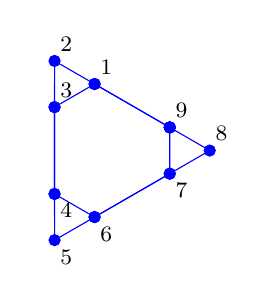
\begin{tikzpicture} 
\begin{axis}[footnotesize,font=\footnotesize
    ,axis equal image, axis lines=none ]
    \addplot[blue,mark=*,domain=40:400,samples=10
    ,nodes near coords={\quad\color{black}\ifnum\coordindex=0\else\coordindex\fi}] 
    ({cos(\x)+0.347*cos(2*\x)}
    ,{sin(\x)-0.347*sin(2*\x)});
    \addplot[blue,mark=*,samples at={40,80,160,200,280,320,40}] 
    ({cos(\x)+0.347*cos(2*\x)}
    ,{sin(\x)-0.347*sin(2*\x)});
\end{axis}
\end{tikzpicture}
\end{wrapfigure}
\begin{example}[\idx{Sierpinski network}] \label{eg:sier2eig}
Consider three triangles formed into a triangle (as shown to the right)---perhaps because triangles make strong structures, or perhaps because of a hierarchical computer\slash social network.
The marginal picture is called a \emidx{network} because it is formed from a set of nodes (the discs) connected by links (the lines).
Let's analyse the matrix used to represent such a network.
 
Form an matrix \(A=\begin{bmatrix} a_{ij} \end{bmatrix}\) of ones if node~\(i\) is connected to node~\(j\);  set the diagonal~\(a_{ii}\) to be minus the number of other nodes to which node~\(i\) is connected; and all other components of~\(A\) are zero.
The symmetry of the matrix~\(A\) follows from the symmetry of the connections: construct the matrix, check it is symmetric, and find the \idx{eigenvalue}s and \idx{eigenspace}s with \script, and their \idx{multiplicity}.
For the computed matrices~\(V\) and~\(D\), check that \(AV=VD\) and also that \(V\)~is an \text{orthogonal matrix.}
\begin{solution} In \script\ use
\setbox\ajrqrbox\hbox{\qrcode{% Sierpinski network
A=[-3 1 1 0 0 0 0 0 1
   1 -2 1 0 0 0 0 0 0
   1 1 -3 1 0 0 0 0 0
   0 0 1 -3 1 1 0 0 0
   0 0 0 1 -2 1 0 0 0
   0 0 0 1 1 -3 1 0 0
   0 0 0 0 0 1 -3 1 1
   0 0 0 0 0 0 1 -2 1
   1 0 0 0 0 0 1 1 -3 ]
A-A'
[V,D]=eig(A)
A*V-V*D
V'*V
}}%
\marginajrbox%
\begin{verbatim}
A=[-3 1 1 0 0 0 0 0 1
   1 -2 1 0 0 0 0 0 0
   1 1 -3 1 0 0 0 0 0
   0 0 1 -3 1 1 0 0 0
   0 0 0 1 -2 1 0 0 0
   0 0 0 1 1 -3 1 0 0
   0 0 0 0 0 1 -3 1 1
   0 0 0 0 0 0 1 -2 1
   1 0 0 0 0 0 1 1 -3 ]
A-A'
[V,D]=eig(A)
\end{verbatim}
To two decimal places so that the results fit the page, the computation may give
\begin{verbatim}
V =
 -0.41  0.51 -0.16 -0.21 -0.45  0.18 -0.40  0.06  0.33
  0.00 -0.13  0.28  0.63  0.13 -0.18 -0.58 -0.08  0.33
  0.41 -0.20 -0.49 -0.42  0.32  0.01 -0.36 -0.17  0.33
 -0.41 -0.11  0.52 -0.42  0.32  0.01  0.14 -0.37  0.33
 -0.00 -0.18 -0.26  0.37 -0.22  0.51  0.36 -0.46  0.33
  0.41  0.53  0.07  0.05 -0.10 -0.51  0.33 -0.23  0.33
 -0.41 -0.39 -0.36  0.05 -0.10 -0.51  0.25  0.31  0.33
  0.00  0.31 -0.03  0.16  0.55  0.34  0.22  0.55  0.33
  0.41 -0.33  0.42 -0.21 -0.45  0.18  0.03  0.40  0.33
D =
 -5.00     0     0     0     0     0     0     0     0
     0 -4.30     0     0     0     0     0     0     0
     0     0 -4.30     0     0     0     0     0     0
     0     0     0 -3.00     0     0     0     0     0
     0     0     0     0 -3.00     0     0     0     0
     0     0     0     0     0 -3.00     0     0     0
     0     0     0     0     0     0 -0.70     0     0
     0     0     0     0     0     0     0 -0.70     0
     0     0     0     0     0     0     0     0 -0.00
\end{verbatim}
The five eigenvalues are \(-5.00\), \(-4.30\), \(-3.00\), \(-0.70\) and~\(0.00\) (to two decimal places).
Three of the eigenvalues are repeated as a consequence of the geometric symmetry in the network (different from the symmetry in the matrix).
The following are \text{the eigenspaces.}
\begin{itemize}
\item Corresponding to eigenvalue \(\lambda=-5\) are eigenvectors \(\sloppy\xv\propto(-0.41,0,0.41,-0.41,0,0.41,-0.41,0,0.41)\); that is, the eigenspace \(\EE_{-5}=\Span\{(-1,0,1,-1,0,1,-1,0,1)\}\).
From \cref{def:eigsymult} the multiplicity of eigenvalue \(\lambda=-5\) is one.

\item Corresponding to eigenvalue \(\lambda=-4.30\) there are two eigenvectors computed by \script.
These two eigenvectors are orthogonal (you should check).
Because these arise as the solutions of the homogeneous system \((A-\lambda I)\xv=\ov\)\,, any (nonzero) linear combination of these is also an eigenvector corresponding to the same eigenvalue. 
That is, the eigenspace
\begin{equation*}
\EE_{-4.30}=\Span\left\{ \begin{bmatrix} 0.51\\-0.13\\-0.20\\-0.11\\-0.18\\0.53\\-0.39\\0.31\\-0.33 \end{bmatrix},\  \begin{bmatrix} -0.16\\0.28\\-0.49\\0.52\\-0.26\\0.07\\-0.36\\-0.03\\0.42 \end{bmatrix} \right\}.
\end{equation*}
Hence the eigenvalue \(\lambda=-4.30\) has multiplicity two.

\item Corresponding to eigenvalue \(\lambda=-3\) there are three eigenvectors computed by \script.
These three eigenvectors are orthogonal (you should check).
Thus the eigenspace
\begin{equation*}
\EE_{-3}=\Span\left\{ 
\begin{bmatrix} -0.21\\0.63\\-0.42\\-0.42\\0.37\\0.05\\0.05\\0.16\\-0.21
\end{bmatrix},\  
\begin{bmatrix} -0.45\\0.13\\0.32\\0.32\\-0.22\\-0.10\\-0.10\\0.55\\-0.45
\end{bmatrix},\ 
\begin{bmatrix} 0.18\\-0.18\\0.01\\0.01\\0.51\\-0.51\\-0.51\\0.34\\0.18
 \end{bmatrix} \right\},
\end{equation*}
and so eigenvalue \(\lambda=-3\) has multiplicity three.

\item Corresponding to eigenvalue \(\lambda=-0.70\) there are two eigenvectors computed by \script.
These two eigenvectors are orthogonal (you should check).
Thus the eigenspace
\begin{equation*}
\EE_{-0.70}=\Span\left\{ \begin{bmatrix} -0.40\\-0.58\\-0.36\\0.14\\0.36\\0.33\\0.25\\0.22\\0.03 \end{bmatrix},\  \begin{bmatrix} 0.06\\-0.08\\-0.17\\-0.37\\-0.46\\-0.23\\0.31\\0.55\\0.40 \end{bmatrix} \right\},
\end{equation*}
and so eigenvalue \(\lambda=-0.70\) has multiplicity two.

\item Lastly, corresponding to eigenvalue \(\lambda=0\) are eigenvectors \(\sloppy\xv\propto(0.33,0.33,0.33,0.33,0.33,0.33,0.33,0.33,0.33)\); 
that is, the eigenspace \(\EE_{0}=\Span\{(1,1,1,1,1,1,1,1,1)\}\),
and so eigenvalue \(\lambda=0\) has multiplicity one.

\end{itemize}
Then check \verb|A*V-V*D| is zero \twodp,
{\small%??
\begin{verbatim}
ans =
  0.00  0.00  0.00  0.00  0.00 -0.00 -0.00  0.00 -0.00
  0.00  0.00 -0.00  0.00 -0.00  0.00 -0.00 -0.00  0.00
  0.00  0.00  0.00  0.00 -0.00 -0.00 -0.00  0.00 -0.00
 -0.00  0.00 -0.00 -0.00  0.00 -0.00  0.00 -0.00  0.00
 -0.00 -0.00  0.00 -0.00  0.00 -0.00 -0.00  0.00 -0.00
  0.00  0.00  0.00 -0.00  0.00  0.00 -0.00  0.00  0.00
 -0.00 -0.00  0.00 -0.00 -0.00  0.00 -0.00 -0.00 -0.00
  0.00  0.00  0.00 -0.00  0.00 -0.00  0.00 -0.00  0.00
  0.00  0.00  0.00  0.00 -0.00 -0.00  0.00 -0.00 -0.00
\end{verbatim}
}
and confirm \(V\)~is orthogonal by checking \verb|V'*V| is the identity \twodp
{\small%??
\begin{verbatim}
ans =
  1.00 -0.00 -0.00  0.00  0.00  0.00 -0.00  0.00  0.00
 -0.00  1.00 -0.00 -0.00  0.00  0.00 -0.00 -0.00 -0.00
 -0.00 -0.00  1.00 -0.00  0.00  0.00 -0.00  0.00  0.00
  0.00 -0.00 -0.00  1.00  0.00 -0.00 -0.00  0.00 -0.00
  0.00  0.00  0.00  0.00  1.00  0.00 -0.00  0.00 -0.00
  0.00  0.00  0.00 -0.00  0.00  1.00 -0.00  0.00 -0.00
 -0.00 -0.00 -0.00 -0.00 -0.00 -0.00  1.00 -0.00  0.00
  0.00 -0.00  0.00  0.00  0.00  0.00 -0.00  1.00  0.00
  0.00 -0.00  0.00 -0.00 -0.00 -0.00  0.00  0.00  1.00
\end{verbatim}
}
\end{solution}
\end{example}


\begin{table}\centering\sl
\rule{\linewidth}{1pt}
\begin{minipage}{\linewidth}
In 1966 \index{Kac, Mark}Mark Kac asked ``Can one hear the shape of the drum?"
That is, from just knowing the eigenvalues of a network such as the one in \cref{eg:sier2eig}, can one infer the connectivity of the network?
The question for 2D drums was answered ``no'' in 1992 by Gordon, Webb and Wolpert who constructed two different shaped 2D drums which have the same set of frequencies of \idx{oscillation}: that is, the same set of eigenvalues.
A challenge for an advanced learner is to find the two smallest connected networks that have different connectivity and yet the same eigenvalues (unit strength connections).
\end{minipage}
\rule{\linewidth}{1pt}
\end{table}

Why write ``the computation may give'' in \cref{eg:sier2eig}?  
The reason is associated with the duplicated eigenvalues.
What is important is the \idx{eigenspace}.
When an eigenvalue of a \idx{symmetric matrix} is duplicated in the diagonal~\(D\) (or triplicated), then there are many choices of eigenvectors that form an \idx{orthonormal basis} (\cref{def:orthobasis}) of the eigenspace (the same holds for \idx{singular vector}s of a duplicated singular value).
Different algorithms may report different orthonormal bases of the same eigenspace.
The bases given in \cref{eg:sier2eig} are just one possibility for \text{each eigenspace.}




\begin{theorem} \label{thm:avvd}
For every \(n\times n\) \idx{square matrix}~\(A\) (not just symmetric),
\hlist\lambda m\ are eigenvalues of~\(A\) with corresponding eigenvectors \hlist\vv m, for some~\(m\) (commonly \(m=n\)), iff \(AV=VD\) for \idx{diagonal matrix} \(D=\diag(\hlist\lambda m)\) and \(n\times m\) matrix \(V=\begin{bmatrix} \vv_1&\vv_2&\cdots&\vv_m \end{bmatrix}\) for nonzero \hlist\vv m.
\end{theorem}

\begin{proof} 
From \cref{def:evecval}, \(\lambda_j\)~are eigenvalues and nonzero~\(\vv_j\) are eigenvectors iff \(A\vv_j=\lambda_j\vv_j\)\,.
Form all the cases \(j=1,2,\ldots,m\) into the one matrix equation
\begin{equation*}
\begin{bmatrix} A\vv_1&A\vv_2&\cdots&A\vv_m \end{bmatrix}
=\begin{bmatrix} \lambda_1\vv_1&\lambda_2\vv_2&\cdots&\lambda_m\vv_m \end{bmatrix}
\end{equation*}
By the definition of matrix products this matrix equation is identical to
\begin{equation*}
A\begin{bmatrix} \vv_1&\vv_2&\cdots&\vv_m \end{bmatrix}
=\begin{bmatrix} \vv_1&\vv_2&\cdots&\vv_m \end{bmatrix}
\begin{bmatrix} \lambda_1&0&\cdots&0
\\0&\lambda_2&&0
\\\vdots&&\ddots&\vdots
\\0&0&\cdots&\lambda_m \end{bmatrix}.
\end{equation*}
Since the matrix of eigenvectors is called~\(V\), and the diagonal matrix of eigenvalues is called~\(D\), this equation is the same as \(AV=VD\)\,.
\end{proof}



\begin{example} 
Use \script\ to compute eigenvectors and the eigenvalues of the (symmetric) matrix
\begin{equation*}
A=\begin{bmatrix} 2&2&-2&0
\\2&-1&-2&-3
\\-2&-2&4&0
\\0&-3&0&1
 \end{bmatrix}.
\end{equation*}
Confirm \(AV=VD\) for the computed matrices.
\begin{solution} 
First compute
\setbox\ajrqrbox\hbox{\qrcode{% eigen-problem
A=[2 2 -2 0
 2 -1 -2 -3
 -2 -2 4 0
 0 -3 0 1]
[V,D]=eig(A)
A*V-V*D
}}%
\marginajrbox%
\begin{verbatim}
A=[2 2 -2 0
  2 -1 -2 -3
 -2 -2 4 0
  0 -3 0 1]
[V,D]=eig(A)
\end{verbatim}
The output is \twodp
\begin{verbatim}
V =
  -0.23   0.83   0.08   0.50
   0.82   0.01  -0.40   0.42
   0.15   0.52  -0.42  -0.72
   0.51   0.20   0.81  -0.23
D =
  -3.80      0      0      0
      0   0.77      0      0
      0      0   2.50      0
      0      0      0   6.53
\end{verbatim}
Hence the eigenvalues are \twodp\ \(\lambda_1=-3.80\), \(\lambda_2=0.77\), \(\lambda_3=2.50\) and \(\lambda_4=6.53\)\,.
From the columns of~\verb|V|, corresponding eigenvectors are \twodp\  
\(\vv_1\propto(-0.23,0.82,0.15,0.51)\),
\(\vv_2\propto(0.83,0.01,0.52,0.20)\),
\(\vv_3\propto(0.08,-0.40,-0.42,0.81)\), and
\(\vv_4\propto(0.50,0.42,-0.72,-0.23)\).
Then confirm \verb|A*V-V*D| is zero:
\begin{verbatim}
ans =
   0.00   0.00   0.00   0.00
   0.00   0.00  -0.00   0.00
  -0.00   0.00  -0.00  -0.00
  -0.00  -0.00  -0.00   0.00
\end{verbatim}
\end{solution}
\end{example}








\subsubsection{Find eigenvalues and eigenvectors by hand}
\label{sec:feebh}

\begin{itemize}
\item Recall from previous study (\cref{thm:2x2det}) that a \(2\times 2\) matrix \(A=\begin{bmat} a&b\\c&d \end{bmat}\) has \idx{determinant} \(\det A=|A|=ad-bc\)\,, and that \(A\)~is not \idx{invertible} \idx{iff} \(\det A=0\)\,.
\item Similarly, although not justified until \cref{ch:ddm}, a \(3\times 3\) matrix \(A=\begin{bmat} a&b&c\\d&e&f\\g&h&i \end{bmat}\) has \idx{determinant} \(\det A=|A|=aei+bfg+cdh-ceg-afh-bdi\)\,, and \(A\)~is not \idx{invertible} iff \(\det A=0\)\,.
\end{itemize}
This section shows these two formulas for a \idx{determinant} are useful for hand calculations on small problems.
The formulas are best remembered via the following diagrams where products along the red lines are subtracted from the sum of products along the blue lines, respectively:
\begin{equation}
\input{dettwothree.ltx}
\label{eq:dets23}
\end{equation}
%(Unfortunately, there is not such a practical pattern for analogous determinants of larger matrices.)
\cref{ch:ddm} extends such determinants to any \idx{size} matrix, and explores more useful properties, but for now this is all the information we need on determinants.


For hand calculation on small matrices (\(2\times 2\) or \(3\times3\)) the key property is the following.
By \cref{def:evecval} eigenvalues and eigenvectors are determined from \(A\xv=\lambda\xv\)\,.  
Rearranging, this equation is equivalent to \((A-\lambda I)\xv=\ov\)\,.  
Both \cref{thm:2x2det} (\(2\times2\) matrices) and \cref{thm:detinv} (general matrices) establish that \((A-\lambda I)\xv=\ov\) has \emph{nonzero} solutions~\xv\ iff the determinant \(\det(A-\lambda I)=0\)\,.
Since eigenvectors must be nonzero, the \idx{eigenvalue}s of a \idx{square matrix} are precisely the solutions of \(\det(A-\lambda I)=0\)\,. 
This reasoning leads to the \text{following procedure.}


\begin{procedure}[eigenvalues and eigenvectors] \label{pro:eeh}
To find by hand \idx{eigenvalue}s and \idx{eigenvector}s of any (small) \idx{square matrix}~\(A\):
\begin{enumerate}
%\item determine the \idx{characteristic polynomial} of~\(A\), \(\det(A-\lambda I)\);
\item find all \idx{eigenvalue}s by solving the \bfidx{characteristic equation} of~\(A\), \(\det(A-\lambda I)=0\)\,;
\item for each \idx{eigenvalue}~\(\lambda\), solve the \idx{homogeneous} matrix-vector equation \((A-\lambda I)\xv=\ov\) to find the corresponding \idx{eigenspace}~\(\EE_\lambda\);
\item write each \idx{eigenspace} as the \idx{span} of a few chosen \idx{eigenvector}s.
% could invoke 'basis' but not yet defined, so use vague 'few'
\end{enumerate}
\end{procedure}
%Since, for an \(n\times n\) matrix, the characteristic polynomial is of \(n\)th~degree in~\(\lambda\), there are \(n\)~eigenvalues (when counted according to multiplicity and allowing complex eigenvalues)

This procedure applies to general matrices~\(A\), as fully established in \cref{sec:eennm}, but this chapter uses it only for small symmetric matrices.
Further, this chapter uses it only as a convenient method to illustrate some properties by hand calculation.
None of the beautiful theorems of the next \cref{sec:sm} for symmetric matrices are based upon this \text{`by-hand' procedure}.


\begin{example} \label{eg:2evals}
Use \cref{pro:eeh} to find the eigenvalues and eigenvectors of the matrix
\begin{equation*}
A=\begin{bmatrix} 1&-\frac12\\-\frac12&1 \end{bmatrix}
\end{equation*}
(this is the matrix illustrated in \cref{eg:eig2sym,eg:eig2pic1}).
\begin{solution} Follow the first two steps of \cref{pro:eeh}.
\begin{enumerate}
\item Solve \(\det(A-\lambda I)=0\) for the eigenvalues~\(\lambda\).
Using~\eqref{eq:dets23},
\begin{equation*}
\det(A-\lambda I)=\begin{vmatrix} 1-\lambda&-\frac12\\
-\frac12&1-\lambda \end{vmatrix}
=(1-\lambda)^2-\tfrac14=0\,.
\end{equation*}
That is, \((\lambda-1)^2=\frac14\)\,.  Taking account of both square roots this quadratic gives \(\lambda-1=\pm\frac12\)\,; that is, \(\lambda=1\pm\frac12=\frac12,\frac32\) are the only two eigenvalues.

\item For eigenvectors, consider the two eigenvalues in turn.
\begin{enumerate}
\item For eigenvalue \(\lambda=\frac12\) solve \((A-\lambda I)\xv=\ov\)\,.  That is,
\begin{equation*}
(A-\tfrac12I)\xv
=\begin{bmatrix} 1-\frac12&-\frac12\\
-\frac12&1-\frac12 \end{bmatrix}\xv
=\begin{bmatrix} \frac12&-\frac12\\
-\frac12&\frac12 \end{bmatrix}\xv
=\ov\,.
\end{equation*}
The first component of this system says \(x_1-x_2=0\)\,; that is, \(x_2=x_1\)\,.  
The second component of this system says \(-x_1+x_2=0\)\,; that is, \(x_2=x_1\) (the same).  
So a general solution for a corresponding eigenvector is \(\xv=(1,1)t\) for any nonzero~\(t\).
That is, the eigenspace \(\EE_{1/2}=\Span \{(1,1)\}\).
\item For eigenvalue \(\lambda=\frac32\) solve \((A-\lambda I)\xv=\ov\)\,.  That is,
\begin{equation*}
(A-\tfrac32I)\xv
=\begin{bmatrix} 1-\frac32&-\frac12\\
-\frac12&1-\frac32 \end{bmatrix}\xv
=\begin{bmatrix} -\frac12&-\frac12\\
-\frac12&-\frac12 \end{bmatrix}\xv
=\ov\,.
\end{equation*}
The first component of this system says \(x_1+x_2=0\)\,, as does the second component\,; that is, \(x_2=-x_1\)\,.  
So a general solution for a corresponding eigenvector is \(\xv=(1,-1)t\) for any nonzero~\(t\).
That is, the eigenspace \(\EE_{3/2}=\Span \{(1,-1)\}\).
\end{enumerate}
\end{enumerate}
\end{solution}
\end{example}




\begin{activity}
Consider the matrix \(A=\begin{bmatrix} 3&2\\2&0 \end{bmatrix}\).  
Use its \idx{characteristic equation} to determine that all its eigenvalues are which of the following?
\actposs[4]{\(-1,4\)}{\(-4,1\)}{\(0,3\)}{\(3,4\)}
\end{activity}




\begin{example} \label{eg:eig3introval}
Use the \idx{determinant}~\eqref{eq:dets23} to confirm that \(\lambda=0,1,3\) are the \emph{only} eigenvalues of the matrix
\begin{equation*}
A=\begin{bmatrix} 1&-1&0\\-1&2&-1\\0&-1&1 \end{bmatrix}.
\end{equation*}
(\cref{eg:eig3sp} already found the eigenspaces corresponding to these three eigenvalues.)
\begin{solution} 
To find all eigenvalues, find all solutions of the characteristic equation \(\det(A-\lambda I)=0\)\,.  
Using~\eqref{eq:dets23},
\begin{align*}
\det(A-\lambda I)
&{}=\begin{vmatrix} 1-\lambda&-1&0\\-1&2-\lambda&-1\\0&-1&1-\lambda \end{vmatrix}
\\&{}=(1-\lambda)^2(2-\lambda)+0+0-0-(1-\lambda)-(1-\lambda)
\\&{}=(1-\lambda)\left[(1-\lambda)(2-\lambda)-2\right]
\\&{}=(1-\lambda)\left[2-3\lambda+\lambda^2-2\right]
\\&{}=(1-\lambda)\left[-3\lambda+\lambda^2\right]
\\&{}=(1-\lambda)(-3+\lambda)\lambda\,.
\end{align*}
So the characteristic equation is \((1-\lambda)(-3+\lambda)\lambda=0\)\,. 
In this factored form we see the \emph{only} solutions are the three eigenvalues \(\lambda=0,1,3\) as previously identified.
\end{solution}
\end{example}



\begin{example} \label{eg:3x3hande}
Use \cref{pro:eeh} to find all eigenvalues and the corresponding \idx{eigenspace}s of the \idx{symmetric matrix}
\begin{equation*}
A=\begin{bmatrix} -2&0&-6\\0&4&6\\-6&6&-9 \end{bmatrix}.
\end{equation*}

\begin{solution} 
Follow the steps of \cref{pro:eeh}.
\begin{enumerate}
\item Solve \(\det(A-\lambda I)=0\) for the eigenvalues.
Using~\eqref{eq:dets23},
\begin{align*}
\det(A-\lambda I)
&= \begin{vmatrix} -2-\lambda&0&-6\\0&4-\lambda&6\\-6&6&-9-\lambda \end{vmatrix}
\\&=(-2-\lambda)(4-\lambda)(-9-\lambda)+0\cdot6\cdot(-6)+(-6)\cdot0\cdot 6
\\&\qquad{}
-(-6)(4-\lambda)(-6)-(-2-\lambda)\cdot6\cdot6-0\cdot0\cdot(-9-\lambda)
\\&=(2+\lambda)(4-\lambda)(9+\lambda)+36(-4+\lambda)+36(2+\lambda)
\\&=-\lambda^3-7\lambda^2+98\lambda
\\&=-\lambda(\lambda^2-7\lambda+98)
\\&=-\lambda(\lambda-14)(\lambda+7).
\end{align*}
This determinant is zero only for the three eigenvalues \(\lambda=0,-7,14\).

\item For eigenvectors, consider the three eigenvalues in turn.
\begin{enumerate}
\item For eigenvalue \(\lambda=0\) solve \((A-\lambda I)\vv=\ov\)\,.  
That is,
\begin{equation*}
(A-0I)\vv
=\begin{bmatrix} -2&0&-6\\0&4&6\\-6&6&-9 \end{bmatrix}\vv
=\begin{bmatrix} -2v_1-6v_3\\4v_2+6v_3\\-6v_1+6v_2-9v_3 \end{bmatrix}
=\ov\,.
\end{equation*}
The first row says \(v_1=-3v_3\)\,, the second row says \(v_2=-\frac32v_3\)\,.  
Substituting these into the left-hand side of the third row gives
\(-6v_1+6v_2-9v_3=18v_3-9v_3-9v_3=0\) for every~\(v_3\) which confirms there are nonzero solutions to form eigenvectors.
Eigenvectors may be written in the form \(\vv=(-3v_3,-\frac32v_3,v_3)\); that is, the eigenspace \(\EE_0=\Span\{(-6,-3,2)\}\).

\item For eigenvalue \(\lambda=7\) solve \((A-\lambda I)\vv=\ov\)\,.  
That is,
\begin{equation*}
(A-7I)\vv
=\begin{bmatrix} -9&0&-6\\0&-3&6\\-6&6&-16 \end{bmatrix}\vv
=\begin{bmatrix} -9v_1-6v_3\\-3v_2+6v_3\\-6v_1+6v_2-16v_3 \end{bmatrix}
=\ov\,.
\end{equation*}
The first row says \(v_1=-\frac23v_3\)\,, 
the second row says \(v_2=2v_3\)\,.  
Substituting these into the left-hand side of the third row gives
\(-6v_1+6v_2-16v_3=4v_3+12v_3-16v_3=0\) for every~\(v_3\) which confirms there are nonzero solutions to form eigenvectors.
Eigenvectors may be written in the form 
\(\vv=(-\frac23v_3,2v_3,v_3)\); that is, the eigenspace \(\EE_7=\Span\{(-2,6,3)\}\).

\item For eigenvalue \(\lambda=-14\) solve \((A-\lambda I)\vv=\ov\)\,.  
That is,
\begin{equation*}
(A+14I)\vv
=\begin{bmatrix} 12&0&-6\\0&18&6\\-6&6&5 \end{bmatrix}\vv
=\begin{bmatrix} 12v_1-6v_3\\18v_2+6v_3\\-6v_1+6v_2+5v_3 \end{bmatrix}
=\ov\,.
\end{equation*}
The first row says \(v_1=\frac12v_3\)\,, 
the second row says \(v_2=-\frac13v_3\)\,.  
Substituting these into the left-hand side of the third row gives
\(-6v_1+6v_2+5v_3=-3v_3-2v_3+5v_3=0\) for every~\(v_3\) which confirms there are nonzero solutions to form eigenvectors.
Eigenvectors may be written in the form 
\(\vv=(\frac12v_3,-\frac13v_3,v_3)\); 
that is, the eigenspace \(\EE_{-14}=\Span\{(3,-2,6)\}\).

\end{enumerate}
\end{enumerate}
\end{solution}
\end{example}



General matrices may have non-real \idx{complex valued} eigenvalues and eigenvectors, as seen in the next example, and for good reasons in some applications.
One of the key results of the next \cref{sec:sm} is to prove that real symmetric matrices always have real eigenvalues and eigenvectors.
There are many applications where this reality \text{is crucial.}


\begin{example} \label{eg:ccevals}
Find the eigenvalues and a corresponding eigenvector for the \idx{non-symmetric matrix} \(A=\begin{bmat} 0&1\\-1&0 \end{bmat}\).

(This example aims to recall basic properties of \idx{complex number}s as a prelude to the proof of the reality of eigenvalues for every symmetric matrix.) 
%It reinforces that matrix symmetry is a crucial part of the next section.



\begin{solution} 
\begin{enumerate}
\item Solve the characteristic equation \(\det(A-\lambda I)=0\) for the eigenvalues~\(\lambda\).
Using~\eqref{eq:dets23},
\begin{equation*}
\det(A-\lambda I)
=\begin{vmatrix} -\lambda&1\\-1&-\lambda \end{vmatrix}
=\lambda^2+1=0\,.
\end{equation*}
That is, \(\lambda^2=-1\)\,.  
Taking square roots we find there are two complex eigenvalues \(\lambda=\pm\sqrt{-1}=\pm \i\) (the upright roman character \index{i@$\i$}\(\i=\sqrt{-1}\) distinguishes it from the integer index~\(i\)).
Despite the appearance of \idx{complex number}s, all our arithmetic, algebra and properties continue to hold.
Thus we proceed to find complex \text{valued eigenvectors.}

There is a \idx{Fundamental Theorem of Algebra} (proved in more advanced courses) that establishes that when real numbers fail us, then complex numbers are always sufficient for all eigenvalues.

\item Consider the two eigenvalues in turn.
\begin{enumerate}
\item For eigenvalue \(\lambda=\i\) solve \((A-\lambda I)\xv=\ov\)\,.  That is,
\begin{equation*}
(A-\i I)\xv
=\begin{bmatrix} -\i&1\\
-1&-\i \end{bmatrix}\xv
=\ov\,.
\end{equation*}
The first component of this system says \(-\i x_1+x_2=0\)\,; that is, \(x_2=\i x_1\)\,.  
The second component of this system says \(-x_1-\i x_2=0\)\,; that is, \(x_2=\i x_1\) (the same).  
So a general corresponding eigenvector is the complex \(\xv=(1,\i)t\) for any nonzero~\(t\).
\item For eigenvalue \(\lambda=-\i\) solve \((A-\lambda I)\xv=\ov\)\,.  That is,
\begin{equation*}
(A+\i I)\xv
=\begin{bmatrix} \i&1\\
-1&\i \end{bmatrix}\xv
=\ov\,.
\end{equation*}
The first component of this system says \(\i x_1+x_2=0\)\,; that is, \(x_2=-\i x_1\)\,.  
The second component of this system says \(-x_1+\i x_2=0\)\,; that is, \(x_2=-\i x_1\) (the same).  
So a general corresponding eigenvector is the complex \(\xv=(1,-\i)t\) for any nonzero~\(t\).
\end{enumerate}
\end{enumerate}
\end{solution}
\end{example}


\cref{eg:ccevals} is a problem that might arise using calculus to describe the dynamics of a mass on a spring.  
Let the displacement of the mass be~\(y_1(t)\) then \idx{Newton's law} says the acceleration \(d^2y_1/dt^2\propto -y_1\)\,, the negative of the displacement; for simplicity, let the constant of proportionality be one.  
Introduce \(y_2(t)=dy_1/dt\) then Newton's law becomes \(dy_2/dt=-y_1\)\,.  
Seek solutions of these two first-order \idx{differential equation}s in the form \(y_j(t)=x_je^{\lambda t}\) and the differential equations become \(x_2=\lambda x_1\) and \(\lambda x_2=-x_1\) respectively.  
Forming into a matrix-vector problem these are
\begin{equation*}
\begin{bmatrix} x_2\\-x_1 \end{bmatrix}
=\lambda\begin{bmatrix} x_1\\x_2 \end{bmatrix}
\iff
\begin{bmatrix} 0&1\\-1&0 \end{bmatrix}\xv=\lambda\xv\,.
\end{equation*}
We need to find the eigenvalues and eigenvectors of the matrix: we derive eigenvalues are \(\lambda=\pm \sqrt{-1}=\pm \i\)\,. 
Physically, such \idx{complex eigenvalue}s represent \idx{oscillation}s in time~\(t\) since, for example, \(e^{\lambda t}=e^{\i t}=\cos t+\i\sin t\) by \idx{Euler's formula}. 








\sectionExercises


\begin{exercise} \label{ex:evecpic} 
Each plot below shows (unit) vectors~\xv\  (blue), and for some matrix the corresponding vectors~\(A\xv\) (red) adjoined. 
Estimate which directions~\xv\ are eigenvectors of matrix~\(A\), and for each eigenvector estimate the corresponding eigenvalue.
\begin{Parts}
\def\eRosesize{small}
\item\eRose{1.5}{-1.0}{-1.0}{1.5}%sym
\answer{\(\vv_1\propto\pm(0.7,0.7)\), \(\lambda_1\approx 0.5\)\,;  and
\(\vv_2\propto\pm(-0.7,0.7)\), \(\lambda_2\approx 2.5\)\,.}

\item\eRose{0.5}{0.4}{1.2}{0.3}
\answer{\(\vv_1\propto\pm(-0.5,0.9)\), \(\lambda_1\approx -0.3\)\,;  and
\(\vv_2\propto\pm(0.6,0.8)\), \(\lambda_2\approx 1.1\)\,.}

\item\eRose{-0.5}{0.2}{1.3}{0.4}
\answer{\(\vv_1\propto\pm(-0.7,0.8)\), \(\lambda_1\approx -0.7\)\,;  and
\(\vv_2\propto\pm(0.2,1)\), \(\lambda_2\approx 0.6\)\,.}

\item\eRose{-0.6}{-0.4}{-0.4}{1.0}%sym
\answer{\(\vv_1\propto\pm(1,-0.2)\), \(\lambda_1\approx -0.7\)\,;  and
\(\vv_2\propto\pm(-0.2,1)\), \(\lambda_2\approx 1.1\)\,.}

\begin{reduce}
\item\eRose{1.0}{0.1}{-1.22}{0.3}
\answer{\(\vv_1\propto\pm(-0.3,1)\), \(\lambda_1\approx 0.7\)\,;  and
no other.}

\item\eRose{0.5}{-0.5}{-0.5}{0.0}%sym
\answer{\(\vv_1\propto\pm(0.5,0.9)\), \(\lambda_1\approx -0.3\)\,;  and
\(\vv_2\propto\pm(-0.9,0.5)\), \(\lambda_2\approx 0.8\)\,.}

\item\eRose{-0.2}{0.8}{-0.2}{1.0}
\answer{\(\vv_1\propto\pm(1,0.2)\), \(\lambda_1\approx -0.1\)\,;  and
\(\vv_2\propto\pm(0.6,0.8)\), \(\lambda_2\approx 0.9\)\,.}
\end{reduce}

\item\eRose{1.1}{-0.0}{0.9}{-0.6}
\answer{\(\vv_1\propto\pm(0,1)\), \(\lambda_1\approx -0.6\)\,;  and
\(\vv_2\propto\pm(0.9,0.5)\), \(\lambda_2\approx 1.1\)\,.}

\item\eRose{-0.15}{0.15}{-0.3}{-0.45}
\answer{There appear to be none.}

\end{Parts}
\end{exercise}



\begin{exercise}
In each case use the \idx{matrix-vector product} to determine which of the given vectors are \idx{eigenvector}s of the given matrix? and for each eigenvector what is the corresponding \idx{eigenvalue}?
\begin{enumerate}
\item \(\begin{bmatrix} 6&2\\3&1 \end{bmatrix}\),\quad
\(\begin{bmatrix}2\\1\end{bmatrix}\), \(\begin{bmatrix}1\\-3\end{bmatrix}\), \(\begin{bmatrix}3\\-2\end{bmatrix}\), \(\begin{bmatrix}-\frac12\\-\frac14\end{bmatrix}\), \(\begin{bmatrix}0\\0\end{bmatrix}\), \(\begin{bmatrix}2\\-3\end{bmatrix}\)
\answer{Corresponding eigenvalues are: 7, 0, n/a, 7, n/a, n/a}

\item \(\begin{bmatrix} -2&1\\3&0 \end{bmatrix}\),\quad
\(\begin{bmatrix}1\\1\end{bmatrix}\), \(\begin{bmatrix}-2\\2\end{bmatrix}\), \(\begin{bmatrix}1\\-1\end{bmatrix}\), \(\begin{bmatrix}1\\3\end{bmatrix}\), \(\begin{bmatrix}0\\0\end{bmatrix}\), \(\begin{bmatrix}-\frac13\\-1\end{bmatrix}\), \(\begin{bmatrix}\frac12\\1\end{bmatrix}\)
\answer{Corresponding eigenvalues are: n/a, -3, -3, 1, n/a, 1, n/a}

\item \(\begin{bmatrix} 3&3&4\\0&-4&0\\-2&-1&-6 \end{bmatrix}\),\quad
\(\begin{bmatrix}4\\0\\-1\end{bmatrix}\), \(\begin{bmatrix}-1\\0\\2\end{bmatrix}\), \(\begin{bmatrix}-2\\6\\-1\end{bmatrix}\), \(\begin{bmatrix}1\\1\\1\end{bmatrix}\), \(\begin{bmatrix}\frac13\\-1\\\frac16\end{bmatrix}\), \(\begin{bmatrix}1\\0\\2\end{bmatrix}\)
\answer{Corresponding eigenvalues are: 2, -5, -4, n/a, -4, n/a}

\item \(\begin{bmatrix} 3&0&0\\2&-5&-3\\-4&-2&0 \end{bmatrix}\),\quad
\(\begin{bmatrix}2\\1\\-1\end{bmatrix}\), \(\begin{bmatrix}0\\-1\\2\end{bmatrix}\), \(\begin{bmatrix}0\\1\\2\end{bmatrix}\), \(\begin{bmatrix}0\\3\\1\end{bmatrix}\), \(\begin{bmatrix}\frac12\\\frac12\\-1\end{bmatrix}\), \(\begin{bmatrix}0\\0\\0\end{bmatrix}\), \(\begin{bmatrix}0\\-1\\-\frac13\end{bmatrix}\)
\answer{Corresponding eigenvalues are: n/a, 1, n/a, -6, 3, n/a, -6}

\begin{reduce}
\item \(\begin{bmatrix} -2&0&0&0\\1&-2&3&-2\\-5&-3&4&-2\\-5&1&-1&0 \end{bmatrix}\),\quad
\(\begin{bmatrix}2\\0\\4\\7\end{bmatrix}\), \(\begin{bmatrix}0\\2\\2\\1\end{bmatrix}\), \(\begin{bmatrix}1\\-2\\2\\-1\end{bmatrix}\), \(\begin{bmatrix}0\\2\\2\\0\end{bmatrix}\), \(\begin{bmatrix}0\\-1\\-1\\0\end{bmatrix}\), \(\begin{bmatrix}1\\0\\2\\1\end{bmatrix}\)
\answer{Corresponding eigenvalues are: -2, 0, n/a, 1, 1, n/a}

\item \(\begin{bmatrix} 5&-4&-1&0\\ 1&0&-1&0\\ -5&8&2&5\\ 4&-4&1&1 \end{bmatrix}\),\quad
\(\begin{bmatrix}2\\0\\4\\1\end{bmatrix}\), \(\begin{bmatrix}1\\1\\1\\-1\end{bmatrix}\), \(\begin{bmatrix}1\\1\\1\\1\end{bmatrix}\), \(\begin{bmatrix}1\\1\\0\\-\frac35\end{bmatrix}\), \(\begin{bmatrix}1\\-\frac12\\3\\3\end{bmatrix}\), \(\begin{bmatrix}0\\\frac12\\1\\1\end{bmatrix}\), \(\begin{bmatrix}-1\\-1\\2\\1\end{bmatrix}\)
\answer{Corresponding eigenvalues are: n/a, 0, n/a, 1, 4, n/a, 3}
\end{reduce}

\end{enumerate}
%\begin{comment} brutal search
%\begin{verbatim}
%format rat
%n=2
%for i=1:10^(n-1)
%A=round(randn(n,n)*3); %A=(A+A')/2;
%[V,D]=eig(A); D=diag(D)';
%if imag(D)==zeros(1,n),
%V=V*diag(1./max(abs(V))); [Vn,Vd]=rat(V,1e-7);
%if max(Vd(:))<10,ADV=[A;D;V], end, end
%end
%\end{verbatim}
%\end{comment}
\end{exercise}




\begin{exercise}  
Use the \script\ function \index{eig()@\texttt{eig()}}\verb|eig()| to determine the eigenvalues and corresponding \idx{eigenspace}s of the following symmetric matrices.
\begin{Parts}
\item  \(\begin{bmatrix} -1 & -\frac{4}{5} & \frac{12}{5} & -2
\\ -\frac{4}{5} & \frac{1}{5} & -\frac{8}{5} & -\frac{12}{5}
\\ \frac{12}{5} & -\frac{8}{5} & -\frac{11}{5} & -\frac{14}{5}
\\ -2 & -\frac{12}{5} & -\frac{14}{5} & 2
\end{bmatrix}\)
\answer{Eigenvalues \( -3,-5,2,5\).}

\item  \(\begin{bmatrix} \frac{7}{5} & -\frac{2}{5} & 0 & -\frac{2}{5}
\\ -\frac{2}{5} & 2 & \frac{2}{5} & 0
\\ 0 & \frac{2}{5} & \frac{13}{5} & \frac{2}{5}
\\ -\frac{2}{5} & 0 & \frac{2}{5} & 2
\end{bmatrix}\)
\answer{Eigenvalues \( 2,3,1\), eigenspace \(\EE_2\) is 2D.}

\begin{reduce}
\item  \(\begin{bmatrix} \frac{30}{7} & \frac{16}{7} & \frac{16}{7} & \frac{4}{7}
\\ \frac{16}{7} & \frac{30}{7} & \frac{16}{7} & \frac{4}{7}
\\ \frac{16}{7} & \frac{16}{7} & \frac{30}{7} & \frac{4}{7}
\\ \frac{4}{7} & \frac{4}{7} & \frac{4}{7} & \frac{15}{7}
\end{bmatrix}\)
\answer{Eigenvalues \(2,9\), eigenspace \(\EE_{2}\) is 3D.}

\item  \(\begin{bmatrix} -\frac{36}{7} & -\frac{8}{7} & \frac{20}{7} & \frac{12}{7}
\\ -\frac{8}{7} & -\frac{6}{7} & -\frac{12}{7} & \frac{20}{7}
\\ \frac{20}{7} & -\frac{12}{7} & -3 & -\frac{32}{7}
\\ \frac{12}{7} & \frac{20}{7} & -\frac{32}{7} & -3
\end{bmatrix}\)
\answer{Eigenvalues \( -3,4,-10\), eigenspace \(\EE_{-3}\) is 2D.}

\item  \(\begin{bmatrix} -2.6 & -2.7 & 5.2 & 2.1
\\ -2.7 & 4.6 & 9.9 & 5.2
\\ 5.2 & 9.9 & -2.6 & 2.7
\\ 2.1 & 5.2 & 2.7 & 4.6
\end{bmatrix}\)
\answer{Eigenvalues \( 2,-13,15,0\).}
\end{reduce}


\item  \(\begin{bmatrix} 1.4 & -7.1 & -0.7 & 6.2
\\ -7.1 & -1.0 & -2.2 & -2.5
\\ -0.7 & -2.2 & -3.4 & -4.1
\\ 6.2 & -2.5 & -4.1 & -1.0
\end{bmatrix}\)
\answer{Eigenvalues \( 11,-8,1\), eigenspace \(\EE_{-8}\) is 2D.}

\item  \(\begin{bmatrix} -1 & 1 & 4 & -3 & 1
\\ 1 & 0 & -2 & 1 & 0
\\ 4 & -2 & 1 & -3 & 0
\\ -3 & 1 & -3 & 2 & -1
\\ 1 & 0 & 0 & -1 & -1
\end{bmatrix}\)
\answer{Eigenvalues  \(-5.1461\), \(-1.6639\), \(-0.7427\), \(0.7676\), \(7.7851\).}

\begin{reduce}
\item  \(\begin{bmatrix} 5 & -1 & 3 & 0 & 0
\\ -1 & -1 & 0 & 0 & -2
\\ 3 & 0 & 1 & 1 & 1
\\ 0 & 0 & 1 & 0 & 0
\\ 0 & -2 & 1 & 0 & -1
\end{bmatrix}\)
\answer{Eigenvalues  \(-3.3693\), \(-1.0170\), \(0.6342\), \(0.9466\), \(6.8055\).}
\end{reduce}


\end{Parts}
%\begin{comment} brutal search
%\begin{verbatim}
%format rat
%v=[1   2   2   4
%  -2   1  -4   2
%  -4   2   2  -1
%  -2  -4   1   2]/5;
%v=[1  4  4  4
%  -4  1 -4  4
%   4 -4 -1  4
%  -4 -4  4  1]/7;
%v=[1   5   5   7
%  -5   1  -7   5
%  -7  -5   5   1
%   5  -7  -1   5]/10;
%n=4
%for i=1:99,
%d=round(randn(1,n)*7);
%[~,j]=sort(rand(1,n)); [~,i]=sort(rand(1,n));
%a=v(i,j)*diag(d)*v(i,j)'; [an,ad]=rat(a,1e-7);
%if max(ad(:))<20,ADV=[a;d], end
%end
%\end{verbatim}
%\end{comment}
\end{exercise}





\begin{exercise}  
For each of the given symmetric matrices, determine all eigenvalues by finding and solving the \idx{characteristic equation} of the matrix.
\begin{Parts}
\item \(\begin{bmatrix} 2&3\\3&2 \end{bmatrix}\)
\answer{\(-1,5\)}
\item \(\begin{bmatrix} 6&\frac{11}2\\\frac{11}2&6 \end{bmatrix}\)
\answer{\(\frac12,\frac{23}2\)}
\item \(\begin{bmatrix} -5&1\\2&-2 \end{bmatrix}\)
\answer{\(-6,-1\)}
\item \(\begin{bmatrix} -5&5\\5&-5 \end{bmatrix}\)
\answer{\(-10,0\)}

\begin{reduce}
\item \(\begin{bmatrix} 5&-4\\-4&-1 \end{bmatrix}\)
\answer{\(-3,7\)}
\item \(\begin{bmatrix} -2&\frac92\\\frac92&10 \end{bmatrix}\)
\answer{\(-\frac72,\frac{23}2\)}
\item \(\begin{bmatrix}6&0&-4
\\0&6&3
\\-4&3&6
 \end{bmatrix}\)
\answer{\(1,6,11\)}
\item \(\begin{bmatrix}-2&4&6
\\4&0&4
\\6&4&-2
 \end{bmatrix}\)
\answer{\(-8,-4,8\)}
\end{reduce}

\item \(\begin{bmatrix}2&-3&-3
\\-3&2&-3
\\-3&-3&2
 \end{bmatrix}\)
\answer{\(-4,5\)(twice)}
\item \(\begin{bmatrix}4&-4&3
\\-4&-2&6
\\3&6&-8
 \end{bmatrix}\)
\answer{\(-13,1,6\)}
\item \(\begin{bmatrix}8&4&2
\\4&0&0
\\2&0&0
 \end{bmatrix}\)
\answer{\(-2,0,10\)}
\item \(\begin{bmatrix}0&0&-3 
\\0&2&0 
\\-3&0&0
 \end{bmatrix}\)
\answer{\(-3,2,3\)}
\end{Parts}
%\begin{comment}brutal search for this and later
%\begin{verbatim}
%format rat
%n=3
%for i=1:10^(n-1)
%A=randn(n,n)*3; A=round(A+A');
%[V,D]=eig(A); D=diag(D)';
%%if D(1)==D(2)|D(2)==D(3),
%V=V*diag(1./max(abs(V)));
%[Dn,Dd]=rat(D,1e-7);
%if max(Dd(:))<10, ADV=[A;D;V], end
%%end
%end
%\end{verbatim}
%\end{comment}
\end{exercise}


\begin{exercise} 
For each symmetric matrix, find the \idx{eigenspace} of the given `eigenvalues' by hand solution of \idx{linear equation}s, or determine from your solution that the given value cannot be an eigenvalue.
\begin{Parts}
\item \(\begin{bmatrix} 1&3\\3&1 \end{bmatrix}\), \(4\), \(-2\)
\answer{\(\EE_4=\Span\{(-1,1)\}\), \(\EE_{-2}=\Span\{(1,1)\}\)}

\item \(\begin{bmatrix} 4&-2\\-2&7 \end{bmatrix}\), \(3\), \(6\)
\answer{\(\EE_3=\Span\{(-1,2)\}\), \(6\)~is not an eigenvalue}

\item \(\begin{bmatrix} -7 & 0 & 2
\\ 0 & -7 & -2
\\ 2 & -2 & -0 \end{bmatrix}\), \(-8\), \(-7\), \(1\)
\answer{\(\EE_{-8}=\Span\{(2,-2,-1)\}\), \(\EE_{-7}=\Span\{(-1,-1,0)\}\), \(\EE_1=\Span\{(1,-1,4)\}\)}

\item \(\begin{bmatrix} 0 & 6 & -3
\\ 6 & 0 & 7
\\ -3 & 7 & 3 \end{bmatrix}\), \(-6\), \(4\), \(9\)
\answer{\(-6\)~is not an eigenvalue, \(\EE_4=\Span\{(3,1,-2)\}\), \(\EE_9=\Span\{(1,3,3)\}\)}

\begin{reduce}
\item \(\begin{bmatrix} 0 & -4 & 2
\\ -4 & 1 & -0
\\ 2 & -0 & 1 \end{bmatrix}\), \(-4\), \(1\), \(2\)
\answer{\(\EE_{-4}=\Span\{(5,4,-2)\}\),
\(\EE_1=\Span\{(0,1,2)\}\),
\(2\)~is not an eigenvalue}

\item \(\begin{bmatrix} 7 & -4 & -2
\\ -4 & 9 & -4
\\ -2 & -4 & 7 \end{bmatrix}\), \(1\), \(4\), \(9\)
\answer{\(\EE_1=\Span\{(1,1,1)\}\),
\(4\)~is not an eigenvalue,
\(\EE_9=\Span\{(1,-2,1)\}\).}
\end{reduce}
\end{Parts}
\end{exercise}



\begin{exercise} 
For each \idx{symmetric matrix}, find by hand all \idx{eigenvalue}s and an \idx{orthonormal basis} for all the corresponding \idx{eigenspace}s.
What is the \idx{multiplicity} of each eigenvalue?
\begin{Parts}
\item \(\begin{bmatrix} -8 & 3
\\ 3 & 0 \end{bmatrix}\)
\answer{\(\EE_{-9}=\Span\{(3,-1)\}\),
\(\EE_{1}=\Span\{(1,3)\}\).
Both eigenvalues have multiplicity one.}

\item \(\begin{bmatrix} 6 & -5
\\ -5 & 6 \end{bmatrix}\)
\answer{\(\EE_{1}=\Span\{(1,1)\}\),
\(\EE_{11}=\Span\{(-1,1)\}\).
Both eigenvalues have multiplicity one.}

\begin{reduce}
\item \(\begin{bmatrix} -2 & -2
\\ -2 & -5 \end{bmatrix}\)
\answer{\(\EE_{-6}=\Span\{(1,2)\}\),
\(\EE_{-1}=\Span\{(-2,1)\}\).
Both eigenvalues have multiplicity one.}

\item \(\begin{bmatrix} 2 & -3
\\ -3 & -6 \end{bmatrix}\)
\answer{\(\EE_{-7}=\Span\{(1,3)\}\),
\(\EE_{3}=\Span\{(-3,1)\}\).
Both eigenvalues have multiplicity one.}

\item \(\begin{bmatrix} -1 & -3 & -3
\\ -3 & -5 & 3
\\ -3 & 3 & -1 \end{bmatrix}\)
\answer{\(\EE_{-7}=\Span\{(1,3,-1)\}\),
\(\EE_{-4}=\Span\{(1,0,1)\}\),
\(\EE_{4}=\Span\{(-3,2,3)\}\).
All eigenvalues have multiplicity one.}

\item \(\begin{bmatrix} -5 & 2 & -2
\\ 2 & -2 & 1
\\ -2 & 1 & -10 \end{bmatrix}\)
\answer{\(\EE_{-11}=\Span\{(2,-1,5)\}\),
\(\EE_{-5}=\Span\{(-2,1,1)\}\),
\(\EE_{-1}=\Span\{(1,2,0)\}\).
All eigenvalues have multiplicity one.}
\end{reduce}

\item \(\begin{bmatrix} 11 & 4 & -2
\\ 4 & 5 & 4
\\ -2 & 4 & 11 \end{bmatrix}\)
\answer{\(\EE_{1}=\Span\{(-1,2,-1)\}\),
\(\EE_{13}=\Span\{(-1,2,5),(2,1,0)\}\).
Eigenvalue \(\lambda=1\) has multiplicity one, whereas \(\lambda=13\) has multiplicity two.}

\item \(\begin{bmatrix} -7 & 2 & 2
\\ 2 & -6 & 0
\\ 2 & 0 & -8 \end{bmatrix}\)
\answer{\(\EE_{-10}=\Span\{(-2,1,2)\}\),
\(\EE_{-7}=\Span\{(-1,2,-2)\}\),
\(\EE_{-4}=\Span\{(2,2,1)\}\).
All eigenvalues have multiplicity one.}

\item \(\begin{bmatrix} 6 & 10 & -5
\\ 10 & 13 & -2
\\ -5 & -2 & -2 \end{bmatrix}\)
\answer{\(\EE_{-5}=\Span\{(5,-2,7)\}\),
\(\EE_{1}=\Span\{(1,-1,-1)\}\),
\(\EE_{21}=\Span\{(3,4,-1)\}\).
All eigenvalues have multiplicity one.}

\item \(\begin{bmatrix}  4 & 3 & 1
\\ 3 & -4 & -3
\\ 1 & -3 & 4 \end{bmatrix}\)
\answer{\(\EE_{-6}=\Span\{(-1,3,1)\}\),
\(\EE_{5}=\Span\{(3,1,0),(-1,3,-10)\}\)
Eigenvalue \(\lambda=-6\) has multiplicity one, whereas \(\lambda=5\) has multiplicity two.}

\end{Parts}
\end{exercise}






\begin{exercise}[\idx{Seven Bridges of K\"onigsberg}]  
The marginal picture shows the abstract \idx{network} of the seven bridges of K\"onigsberg during the time of \idx{Euler}: the small disc nodes represent the islands of K\"onigsberg; the lines between represent the seven different bridges that connect the islands.
\marginpar{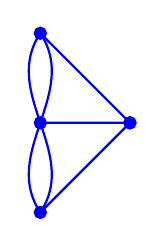
\begin{tikzpicture}
\begin{axis}[axis equal image, axis lines=none,footnotesize]
\addplot[blue,thick,mark=*] coordinates {(0,0)(1,0)(0,1)(1,0)(0,-1)};
\addplot[blue,smooth,thick,domain=-1:1,no marks] ({(x-x^3)/3},{x});
\addplot[blue,smooth,thick,domain=-1:1,no marks] ({-(x-x^3)/3},{x});
\end{axis}
\end{tikzpicture}}%
This abstract network is famous for its role in founding the theory of such networks, but this exercise addresses an aspect relevant to well used web search software.
Number the nodes from~\(1\) to~\(4\).
Form the \(4\times 4\) \idx{symmetric matrix} of the number of lines from each node to the other nodes (and zero for the number of lines from a node to itself)---called the \idx{adjacency matrix}.
Use \script\ function \index{eig()@\texttt{eig()}}\verb|eig()| to find the eigenvalues and eigenvectors for this matrix.
Analogous to well known web search software, identify the largest eigenvalue and a corresponding eigenvector:  then we choose to rank the importance of each node in order of the \idx{magnitude} of the component in the corresponding~eigenvector.
\answer{Number the nodes as you like, say 1=top, 2=centre, 3=right, and 4=bottom.
Then the matrix is \(\protect\begin{bmat} 0&2&1&0
\\2&0&1&2
\\1&1&0&1
\\0&2&1&0 \protect\end{bmat}\).
Eigenvalues are \(-2.86,-0.77,0.00,3.63\) \twodp\ and an eigenvector corresponding to the largest~\(3.63\) is \((0.46,0.63,0.43,0.46)\).
Thus rank the centre left node as the most important, the right node is least important, and the top and bottom nodes equal second importance.}
\end{exercise}



\begin{exercise} 
For each of the following \idx{network}s:\footnote{Although a well known web search engine computes eigenvectors for all the web pages on the internet, it uses an approximate iterative algorithm more suited to the mind-boggingly vast size of the internet.}
\begin{itemize}
\item label the nodes; 
\item construct the symmetric \idx{adjacency matrix}~\(A\) such that \(a_{ij}\)~is one if node~\(i\) is linked to node~\(j\), and \(a_{ij}\)~is zero otherwise (and zero on the diagonal);
\item in \script\ use \index{eig()@\texttt{eig()}}\verb|eig()| to find all eigenvalues and eigenvectors;
\item rank the `importance' of the nodes from the \idx{magnitude} of their component in the eigenvector corresponding to the largest (most positive) eigenvalue.
\end{itemize}
 

\newcommand{\netwk}[2]{\begin{tikzpicture}
\begin{axis}[axis equal image, axis lines=none,small]
\addplot[blue,only marks,mark=*,samples=#1+1,domain=0:360]  ({cos(x)},{sin(x)});
\foreach \p in {1,2,...,#2} {
    \addplot[blue,thick,samples=2,domain={rnd}:{rnd}]   
    ({cos(360*round(x*#1)/#1)},{sin(360*round(x*#1)/#1)});
    }
\end{axis}
\end{tikzpicture}}
\pgfmathsetseed{1138}% set seed so graphs remain fixed
\begin{Parts}
\item\netwk5{12}
\item\hspace*{-1em}%%%%%%%%%%%%%%%%%%??
\netwk6{20}
\item\netwk8{20}
\item\netwk9{20}
\end{Parts}
\end{exercise}



\begin{comment}
Could also give some examples dressed as ODEs (leave to the ODEs in EigGen) or internal stresses.
\end{comment}


\begin{exercise}  
In a few sentences, answer\slash discuss each of the following.
\begin{enumerate}
\item In an \svd, \(\usv\), what is important about singular vectors for which \(\uv_j=\pm \vv_j\)?

\item What fundamental geometric question corresponds to seeking eigenvalues and eigenvectors?

\item Why do we require eigenvectors to be nonzero?

\item For a symmetric matrix, how do its singular values compare to its eigenvalues?

\item What geometric reason underlies the simplicity of the eigenvalues and eigenvectors of diagonal matrices?

\item How does the concept of an eigenspace follow from that of eigenvalues and eigenvectors?

\item How did the concept of multiplicity of eigenvalues for symmetric matrices arise?

\item How is it that complex eigenvalues can arise for real matrices?

\end{enumerate}
\end{exercise}

\begin{comment}%{ED498555.pdf}
why, what caused X?
how did X occur?
what-if? what-if-not?
how does X compare with Y?
what is the evidence for X?
why is X important?
\end{comment}


\index{eigenvalue|)}
\index{eigenvector|)}
